\documentclass[letterpaper,twocolumn,superscriptaddress,showkeys]{revtex4}
\usepackage[utf8]{inputenc}
\usepackage{color,dcolumn,graphicx,hyperref}
\hypersetup
{
    colorlinks = true, linkcolor = blue, citecolor = blue, urlcolor = blue,
}

\begin{document}

\title{Open Preprints in Ecology \& Evolution}

\author{Philippe Desjardins-Proulx}
\email[E-mail: ]{philippe.d.proulx@gmail.com}
\affiliation{Theoretical Ecosystem Ecology laboratory, Universit\'e du Qu\'ebec \`a Rimouski, Canada.}
\affiliation{Quebec Center for Biodiversity Science, McGill University, Canada.}
\affiliation{D\'epartement des sciences biologiques, Universit\'e du Qu\'ebec \`a Montr\'eal, Canada.}

\author{Ethan P. White}
\affiliation{Departement of Bology, Utah State University, United-States of America.}

\author{Timoth\'ee Poisot}
\affiliation{Theoretical Ecosystem Ecology laboratory, Universit\'e du Qu\'ebec \`a Rimouski, Canada.}
\affiliation{Quebec Center for Biodiversity Science, McGill University, Canada.}
\affiliation{International Network for Next-Generation Ecology.}

\author{Dominique Gravel}
\affiliation{Theoretical Ecosystem Ecology laboratory, Universit\'e du Qu\'ebec \`a Rimouski, Canada.}
\affiliation{Quebec Center for Biodiversity Science, McGill University, Canada.}

\keywords{Publishing; arXiv; Green Open Access.}

\begin{abstract}

...
 
\end{abstract}

\maketitle

\section{The case for open preprints}

We will highlight advantages for both scientists and publishers.

The first and most often discussed advantage is speed \ref{fig:map}.

%% Allows papers to be cited earlier (greater immediacy)

%% Essentially an open equivalent to sharing preprints between colleagues.

%% @Tim: how can it improve the review process?

\begin{figure}[ht!] \centering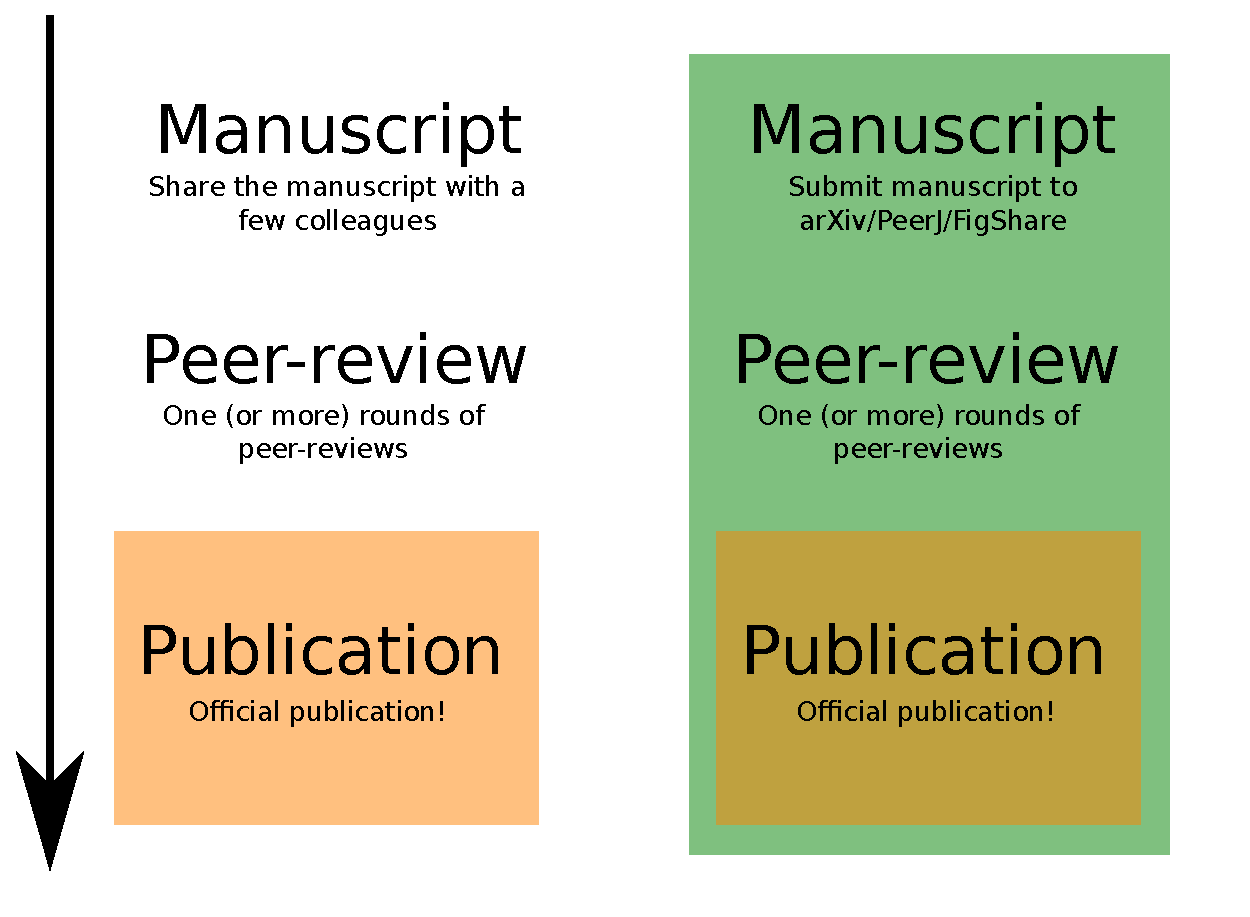
\includegraphics[width=0.50\textwidth]{map.pdf}
\caption { It can take several months, and even a few years, before a submitted
paper is officially published. During this time, few people are aware of the
research that has been done. With public preprint servers, the science is
immediately available and can be openly discussed, analysed, and integrated into
current research. It benefits both science and publishers. Both want the papers
to be well-known and cited, and public preprints make it possible to integrate
research even before publication, improving immediacy.  } \label{fig:map}
\end{figure}

Preprint servers also establish priority in a fair way. Some manuscript will
spend much more time in the review process. Public preprints server offer a much
fairer way to establish intellectual priority By making the manuscript available
when it is ready. Surprisingly, there is perception in biology that public
preprints make it easier to steal ideas, as if scientific ideas only took form
in published material. Mathematicians and physicists have embraced arXiv in part
to establish priority in a fair way\cite{cal12}.

\section{Preprints, Ecology \& Evolution}

While the practice is still rare, preprints are becoming more common in
biological sciences, which is experiencing faster growth in arXiv submission
than any other fields \cite{cal12}. Also, most scientific journals are
preprint-friendly: Nature, PLOS, BMC, PNAS, Science (mostly)
\ref{table:policies}, and all the journals from Elsevier and Springer. Very
recently, the Ecological Society of America recently changed its policy to allow
public preprints (REF). In our field, very few scientific publications will not
consider a manuscript submitted to arXiv. Many ecology \& evolution journals
adopt a ``by default'' hostile attitude towards preprints, mostly due to the
lack of clear policy of the publishers. As an example, Wiley-Blackwell, which
publishes some of the leading journal in the field, has no official policy on
the subject.

\begin{table*}
    \centering
    \begin{tabular}{|ll|}
    \hline
    Publisher                                   & Policy \\
    \hline
    Springer                            	& Accept \\
    BMC                                 	& Accept \\
    Elsevier                            	& Accept \\
    Nature Publishing Group             	& Accept \\
    Public Library of Science           	& Accept \\
    Royal Society                       	& Accept \\
    National Academy of Science (USA)           & Accept \\
    Science                             	& Accept/Ambiguous \\
    Wiley-Blackwell                       	& No general policy \\
    Ecological Society of America       	& Refuse \\
    British Ecological Society                  & ? \\
    \hline
    \end{tabular}
    \caption{Policies for important publishers in ecology and evolution.}
    \label{table:policies}
\end{table*}

\section{Current offer}

% Short paragraphs on the current open preprint repositories.

\subsection{arXiv}

arXiv (\href{http://arxiv.org/}{http://arxiv.org/})

arXiv is funded by a network of universities.

\subsection{Figshare}

Figshare (\href{http://figshare.com/}{http://figshare.com/})

All figshare content (article, figures, datasets) have a unique digital object
identifier (DOI) like any journal article.

\subsection{PeerJ}

% Ethan P. White's section

\subsection{F1000Research}

% Not really the same, but worth mentionning.

\section{Conclusion}

% A short paragraph to conclude.

Responding to the rumour that they refused manuscripts submitted to arXiv,
Nature responded that ``Nature never wishes to stand in the way of communication
between researchers. We seek rather to add value for authors and the community
at large in our peer review, selection and editing'' \cite{nat05}.

\newpage
\bibliography{refs}
\bibliographystyle{plain}

\end{document}

